\subsection{Subsystem Integration}
\label{sec:subsystem_integration}
The integration of all the subsystems is centered around the control subsystem. In the following sections, the team will discuss how these integrations will occur as the design process was centered around creating individual black boxes for each system to work against.

% TODO: Scott look this WHOLE SUBSECTION over and check if it's accurate.
\subsubsection{Sensing}
The sensing subsystem has three key components for the control subsystem to interact with: the linear rail and carriage the spectrometer is mounted to, the laser generating photons for the spectrometer to receive, and the spectrometer itself.

\paragraph{Linear Rail and Carriage} The spectrometer will be mounted to a carriage that may slide back and forth on the linear rail. The position of the carriage on the linear rail determines the wavelength of light sampled, and therefore the wavelength can be interpolated by the position of the stepper motor controlling the spectrometer carriage. It is a natural conclusion that the microcontroller will be able to direct the spectrometer to measure a specific wavelength by moving the stepper motor a certain number of predetermined steps. The microcontroller will sample the entire spectral range and compile this data to prepare to send to the web subsystem for processing.
% TODO: Scott please add how to calculate displacement on the linear rail from the wavelength we are trying to sample
\begin{equation}
    \label{equation:wavelen-dist}
\end{equation}

% TODO: SCOTT fix this paragraph, below the fiber optic we have no clue how you plan on making this work
\paragraph{Laser} The laser mounted to the Carriage will be commanded to power on by the microcontroller whenever the microcontroller wishes to obtain a sample from the spectrometer. The laser itself draws a minimal amount of current and is compatible with the voltages regulated and output by the microcontroller, and will simply be connected to one of the microcontroller's GPIO pins.

\paragraph{Spectrometer} The spectrometer itself will be stationary relative to the spectrometer's carriage. The spectrometer is a passive instrument that generates current depending on the flux density on the sensor. Due to the position of the spectrometer, this flux density is based on the strength of the specific wavelength emission. This current is connected to the sensing subsystem circuitry described in \ref{sec:sensing_subsystem}. This circuitry will proportionally convert the current to a voltage, and the output of the circuit will be connected to an analog-configured pin of the microcontroller, which will be taken as an input to the microcontroller's analog-to-digital converter. The ADC will convert the voltage to a value able to be measured in programming. The current (and by extension, voltage) level measured will be paired with the wavelength and transmitted by the MCU to the Amazon EC2 instance.

% TODO: Justin look this WHOLE SUBSECTION over and check if it's accurate.
\subsubsection{Power} The charge controller will deliver voltage of the battery to the microcontroller via

\subsubsection{Web}
The web and control subsystems interact via two way WebSocket protocol (\ref{websocket_protocol}), which will utilize TCP (\ref{tcp_standard}) as the transport layer protocol. Section \ref{sec:controller_subsystem} talks about the format of the raw texts in the packets. The web subsystem will be deployed to a fixed domain so the memory of the control system can use a fixed host for the Socket server. The socket server will always start by processing the address information of the incoming socket, and grabbing previous data from the database accordingly. The socket server will process the data, storing it in the database for reporting on later. If necessary, the socket server will send a request to the plant bed to do some function. This is laid out in \autoref{fig:web-control-sequence}.

\begin{figure}[H]
    \caption{Web--Plant Bed Socket Integration Sequence Diagram}
    \centering
    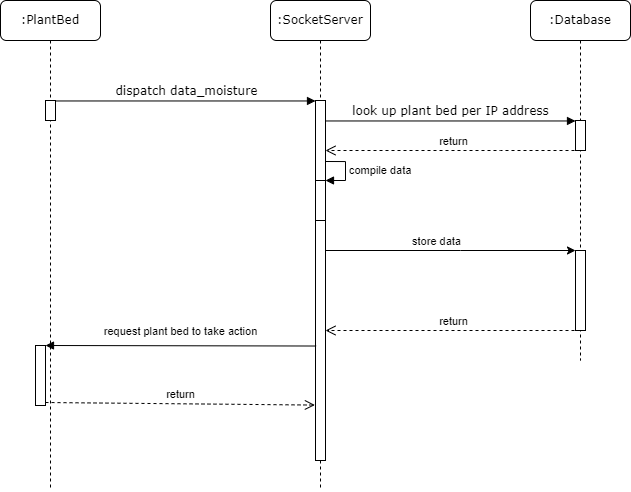
\includegraphics[width=.75\textwidth]{images/web-control-integration-sequence.png}
    \label{fig:web-control-sequence}
\end{figure}

